\documentclass{eeleyes}

\usepackage{fancyhdr}
\pagestyle{fancy}
\fancyhead[lcr]{}
\fancyhead[l]{Eli Griffiths}
\fancyhead[c]{MATH $140$C}
\fancyhead[r]{HW \#$1$}

\begin{document}

\section*{Problem 1}
\begin{proof}
    \hfill
    \begin{enumerate}[label=\roman*)]
        \item Clearly $B \subseteq A \cup B$. Let $x \in A \cup B$. If $x \in B$, then trivially $x \in B$. Consider the case when $x \notin B$. Then $x \in A$. Since $A \subset B$, it follows $x \in B$. Therefore $A \cup B \subseteq B \implies A \cup B = B$.
        \item Clearly $A \cap B \subseteq A$. Let $x \in A$. Since $A \subset B$, $x \in B$ meaning $x \in A \cap B$. Therefore $A \subseteq A \cap B \implies A \cap B = A$. \qedhere
    \end{enumerate}
\end{proof}

\section*{Problem 2}
\begin{enumerate}[label=\alph*)]
    \item $(2, 1, -3) + P = (0, 2, 4) \implies P = (0, 2, 4) - (2, 1, -3) = (-2, 1, 7)$

    \item $\begin{aligned}[t]
        (1, -1, 4) + 2P = 3P + (2, 0, 5) \implies P &= (1, -1, 4) - (2, 0, 5)  \\
        &= (-1, -1, -1)
        \end{aligned}$

\end{enumerate}

\section*{Problem 3}
Adding the equations gives
\[
\begin{aligned}
    3P + Q &= (1, 0, 1, -4) \\
    P - Q &= (2, 1, 2, 3)
\end{aligned} 
\implies 
4P = (3, 1, 3, -1) \implies P = \qty(\frac{3}{4}, \frac{1}{4}, \frac{3}{4}, -\frac{1}{4})
.\]
which when plugged into the second equation
\[
    Q = P - (2,1,2,3) = \qty(-\frac{5}{4}, -\frac{3}{4}, -\frac{5}{4}, -\frac{13}{4})
.\]

\section*{Problem 4}
Yes. Choosing $p = (4,5,-3)$ gives $p \cdot A = 4 + 5 - 9 = 0$ and $p \cdot B = 8 - 5 - 3 = 0$.

\section*{Problem 5}
Let $p = (x,y)$.
\begin{enumerate}[label=\alph*)]
    \item $\begin{aligned}[t] 
            |p| < |p - A| &\implies x^2 + y^2 < (x - 4)^2 + (y - 2)^2  \\
                          &\implies 0 < -8x + 16 - 4y + 4 \\
                          &\implies y < -2x + 5
    \end{aligned}$

    \begin{center}
        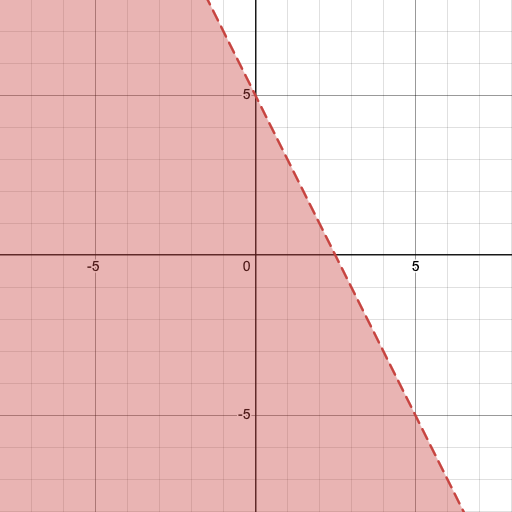
\includegraphics[width=0.4\linewidth]{figures/problem5_a.png}
    \end{center}

    \item The statement is the same as saying the distance from $(0,0)$ to $p$ to $A$ is contant, which by definition is an ellipse with foci $(0,0)$ and $A$ and constant distance $6$. Note this is a non empty set of points since $p = (0,2)$ works.

    \begin{center}
        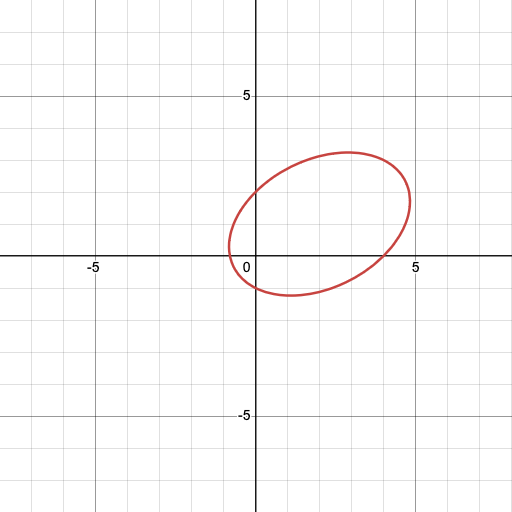
\includegraphics[width=0.4\linewidth]{figures/problem5_b.png}
    \end{center}

    \item No such points in the plane satisfy this. The smallest possible sum is achieved when $p$ is on the line between $(0,0)$ and $A$ (derived from the equations similarity to an ellipse but the point can be on the interior), but this gives a total distance of $|A| = 2 \sqrt{5} > 4$. Thus the graph would be empty

    \begin{center}
        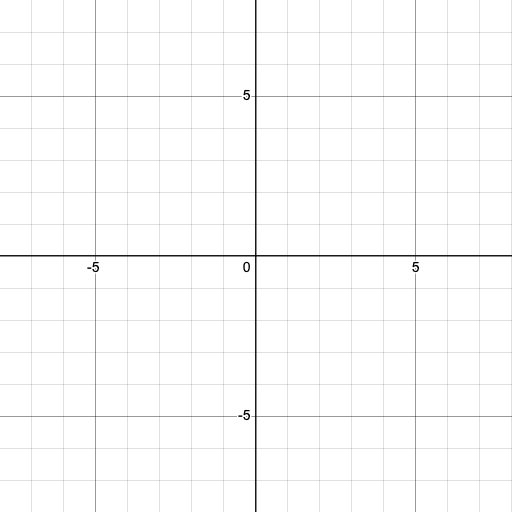
\includegraphics[width=0.4\linewidth]{figures/problem5_c.png}
    \end{center}
\end{enumerate}

\section*{Problem 6}
\begin{proof}
    We proceed with induction on $n$. Consider the base case $n = 1$. Trivially $|p_1| \leq |p_1|$. Fix $n \in \N$ and assume that the statements holds. Consider the $n+1$ case. Note that if $s = p_{n+1} + p_{n}$ that
    \begin{align*}
        \qty|p_1 + \ldots + p_{n} + p_{n+1}| &= \qty|p_1 + \ldots + p_{n-1} + s| \\
                                             &\leq \qty|p_1| + \ldots + \qty|p_{n-1}| + \qty|s| \tag{$\star$} \\
                                             &\leq \qty|p_1| + \ldots + \qty|p_{n-1}| + \qty|p_{n}| + \qty|p_{n+1}|
    \end{align*}
    where $(\star)$ follows from the induction hypothesis and the last line from the triangle inequality applied to $|s|$. Thus the $n+1$ case holds, hence the statement holds for all $n$.
\end{proof}

\section*{Problem 7}
\begin{proof}
    By triangle inequality
    \[
        |p| = |(p-q) + q| \leq |p-q| + |q| \implies |p-q| \geq |p| - |q|
    \]
    which was to be shown.
\end{proof}

\section*{Problem 8}
\begin{proof}
\begin{enumerate}[label=\alph*)]
    \item Note that since $|u|, |v|, |w| > 0$, $(|u| + |v| + |w|)^2 \geq |u|^2 + |v|^2 + |w|^2$ meaning
        \[
            |p|^2 = u^2 + v^2 + w^2 = |u|^2 + |v|^2 + |w|^2 \leq (|u| + |v| + |w|)^2
        .\]
        Rooting both sides then gives $|p| \leq |u| + |v| + |w|$.
        
    \item Since $|p|^2 = u^2 + v^2 + w^2$ and $u^2, v^2, w^2 \geq 0$
        \begin{alignat*}{11}
            |p|^2 &\geq\; &&u^2 &&= |u|^2 &&\implies &&|u| &&\leq |p| \\
            |p|^2 &\geq\; &&v^2 &&= |v|^2 &&\implies &&|v| &&\leq |p| \\
            |p|^2 &\geq\; &&w^2 &&= |w|^2 &&\implies &&|w| &&\leq |p| \\
        \end{alignat*}
\end{enumerate}
\end{proof}

\section*{Problem 9}
\subsection*{Intersections are Convex}
\begin{proof}
    Let $A, B \subseteq \R^n$ be convex and $x,y \in A \cap B$. Then $x,y \in A$ and $x,y \in B$. Since both sets are convex, for all $\lambda \in (0,1)$
    \begin{align*}
        \lambda x + (1-\lambda) y \in A \\
        \lambda x + (1-\lambda) y \in B
    \end{align*}
    Therefore $\lambda x + (1 - \lambda) y \in A \cap B$, hence $A \cap B$ is convex.
\end{proof}

\subsection*{Unions arent always Convex}
\begin{proof}
    Note that any singleton $\qty{x} \subseteq \R^n$ is convex since $\lambda x + (1-\lambda) x = x \in \qty{x}$. However, for $x \neq y$, $\qty{x} \cup \qty{y}$ cannot be convex, otherwise $\frac{1}{2} (x+y) \in \qty{x,y}$ which would imply $x = y$.
\end{proof}

\end{document}
